\documentclass{WileyMSP-template}

\begin{document}


\pagestyle{fancy}
\rhead{\includegraphics[width=2.5cm]{vch-logo.png}}


\title{Metamaterial-enabled ultrasound wireless power harvesting\\ through a metallic barrier }

\maketitle



% Author: Please give full first and last names for authors and include * after the name of all corresponding authors
\author{Jun Ji}
\author{Hyeonu Heo}
\author{Jiaxin Zhong}
 % \altaffiliation[Also at ]{Physics Department, XYZ University.}%Lines break automatically or can be forced with \\
\author{Mourad Oudich}%
\author{Yun Jing*}

% Dedication
% \dedication{J.J., H.H., and J.Z equally contributed to this work. }

% Affiliations: Please provide adacemic titles (Prof. or Dr.) for all authors where applicable, and include an institutional email address for all corresponding authors
\begin{affiliations}
J. Ji, Dr. H. Heo, Dr. J. Zhong, Prof. M. Oudich, Prof. Y. Jing \\

Graduate Program in Acoustics, The Pennsylvania State University, University Park, PA 16802, USA

Email Address: jing.yun@psu.edu

Prof. M. Oudich \\
Universite de Lorraine, CNRS, Institut Jean Lamour, F-54000 Nancy, France



\end{affiliations}


% Keywords: Please provide a minimum of three and a maximum of seven keywords, separated by commas

\keywords{acoustic metamaterials, wireless power harvesting, ultrasound transmission enhancement}



% Abstract should be written in the present tense and impersonal style (i.e., avoid we), and be at most 200 words long
\begin{abstract}

Please insert your abstract here

\end{abstract}

% Text: Please use section headings and subheadings as specified below. For communications, all section headings apart from Experimental Section should be removed
% Please make the first reference to a display item bold: \textbf{Figure 1}
% Do not abbreviate Figure, Equation, etc.; display items are always singular, i.e., Figure 1 and 2.
% Equations are always singular, i.e., Equation 1 and 2, and should be inserted using the {equation} environment, not as graphics
% Please do not use footnotes in the text, additional information can be added to the Reference list.

\justifying
\section{Introduction}

Through-metal-wall ultrasonic power delivery has become an exciting field of research, as metal barriers prevent the use of electromagnetic wireless power transfer due to Faraday shielding effects\cite{yang2015through}. Conventional ultrasonic power delivery utilizes a pair of PZT ultrasound transducers coupled to a metal barrier through a coupling layer. The main limitation of PZT-based system is that they require direct coupling of piezoelectric transducers with metal walls to provide a good acoustic transmission path. Poor coupling will introduce severe impedance mismatch over the acoustic-electric channel and cause the power transfer efficiency to decrease rapidly. 
\\Acoustic metamaterials \cite{cummer2016controlling} are artificial structures that are capable of controlling the propagation of sound in unconventional ways, and have led to interesting phenomena such as acoustic cloaking, acoustic subwavelength imaging, and acoustic unidirectional transparency. Among them, complementary acoustic metamaterials have been utilized to achieve strong transmission through a solid skull, and theoretically through a metal wall as long as one can design a metamaterial layer satisfying the required negative properties. However, the membrane-based complementary metamaterials usually are not sufficiently durable, which become issues in practical implementation. Time-reversal based techniques have also been used to dedign holographic lenses with tailored phase patterns. However, they mainly aim at reconstructing the distorted transmitted field, and the energy transmission improvement through a plastic skull may not work for through-metal-wall power delivery. More recently, an inversely optimized auxiliary meta-lens has been proposed to assist the power transmission through a 1.8mm thick metal wall at 200 kHz. However, they used an inverse design method by optimizing geometrical parameters of meta-lens in COMSOL, which may not be applicable to general applications. 
\\In this work, we proposed a deterministic method, which is based on band structure and transmission analysis, to design an ultrasonic pillar-based metamaterial, and the vertical elongation mode of the metamaterial is utilized for through-metal-wall power delivery. 

%\subsubsection{First Sub Subsection}
%\threesubsection{First lowest-level subsection}

\section{Results}
\subsection{Pillar-based acoustic metamaterial}



\begin{figure}
  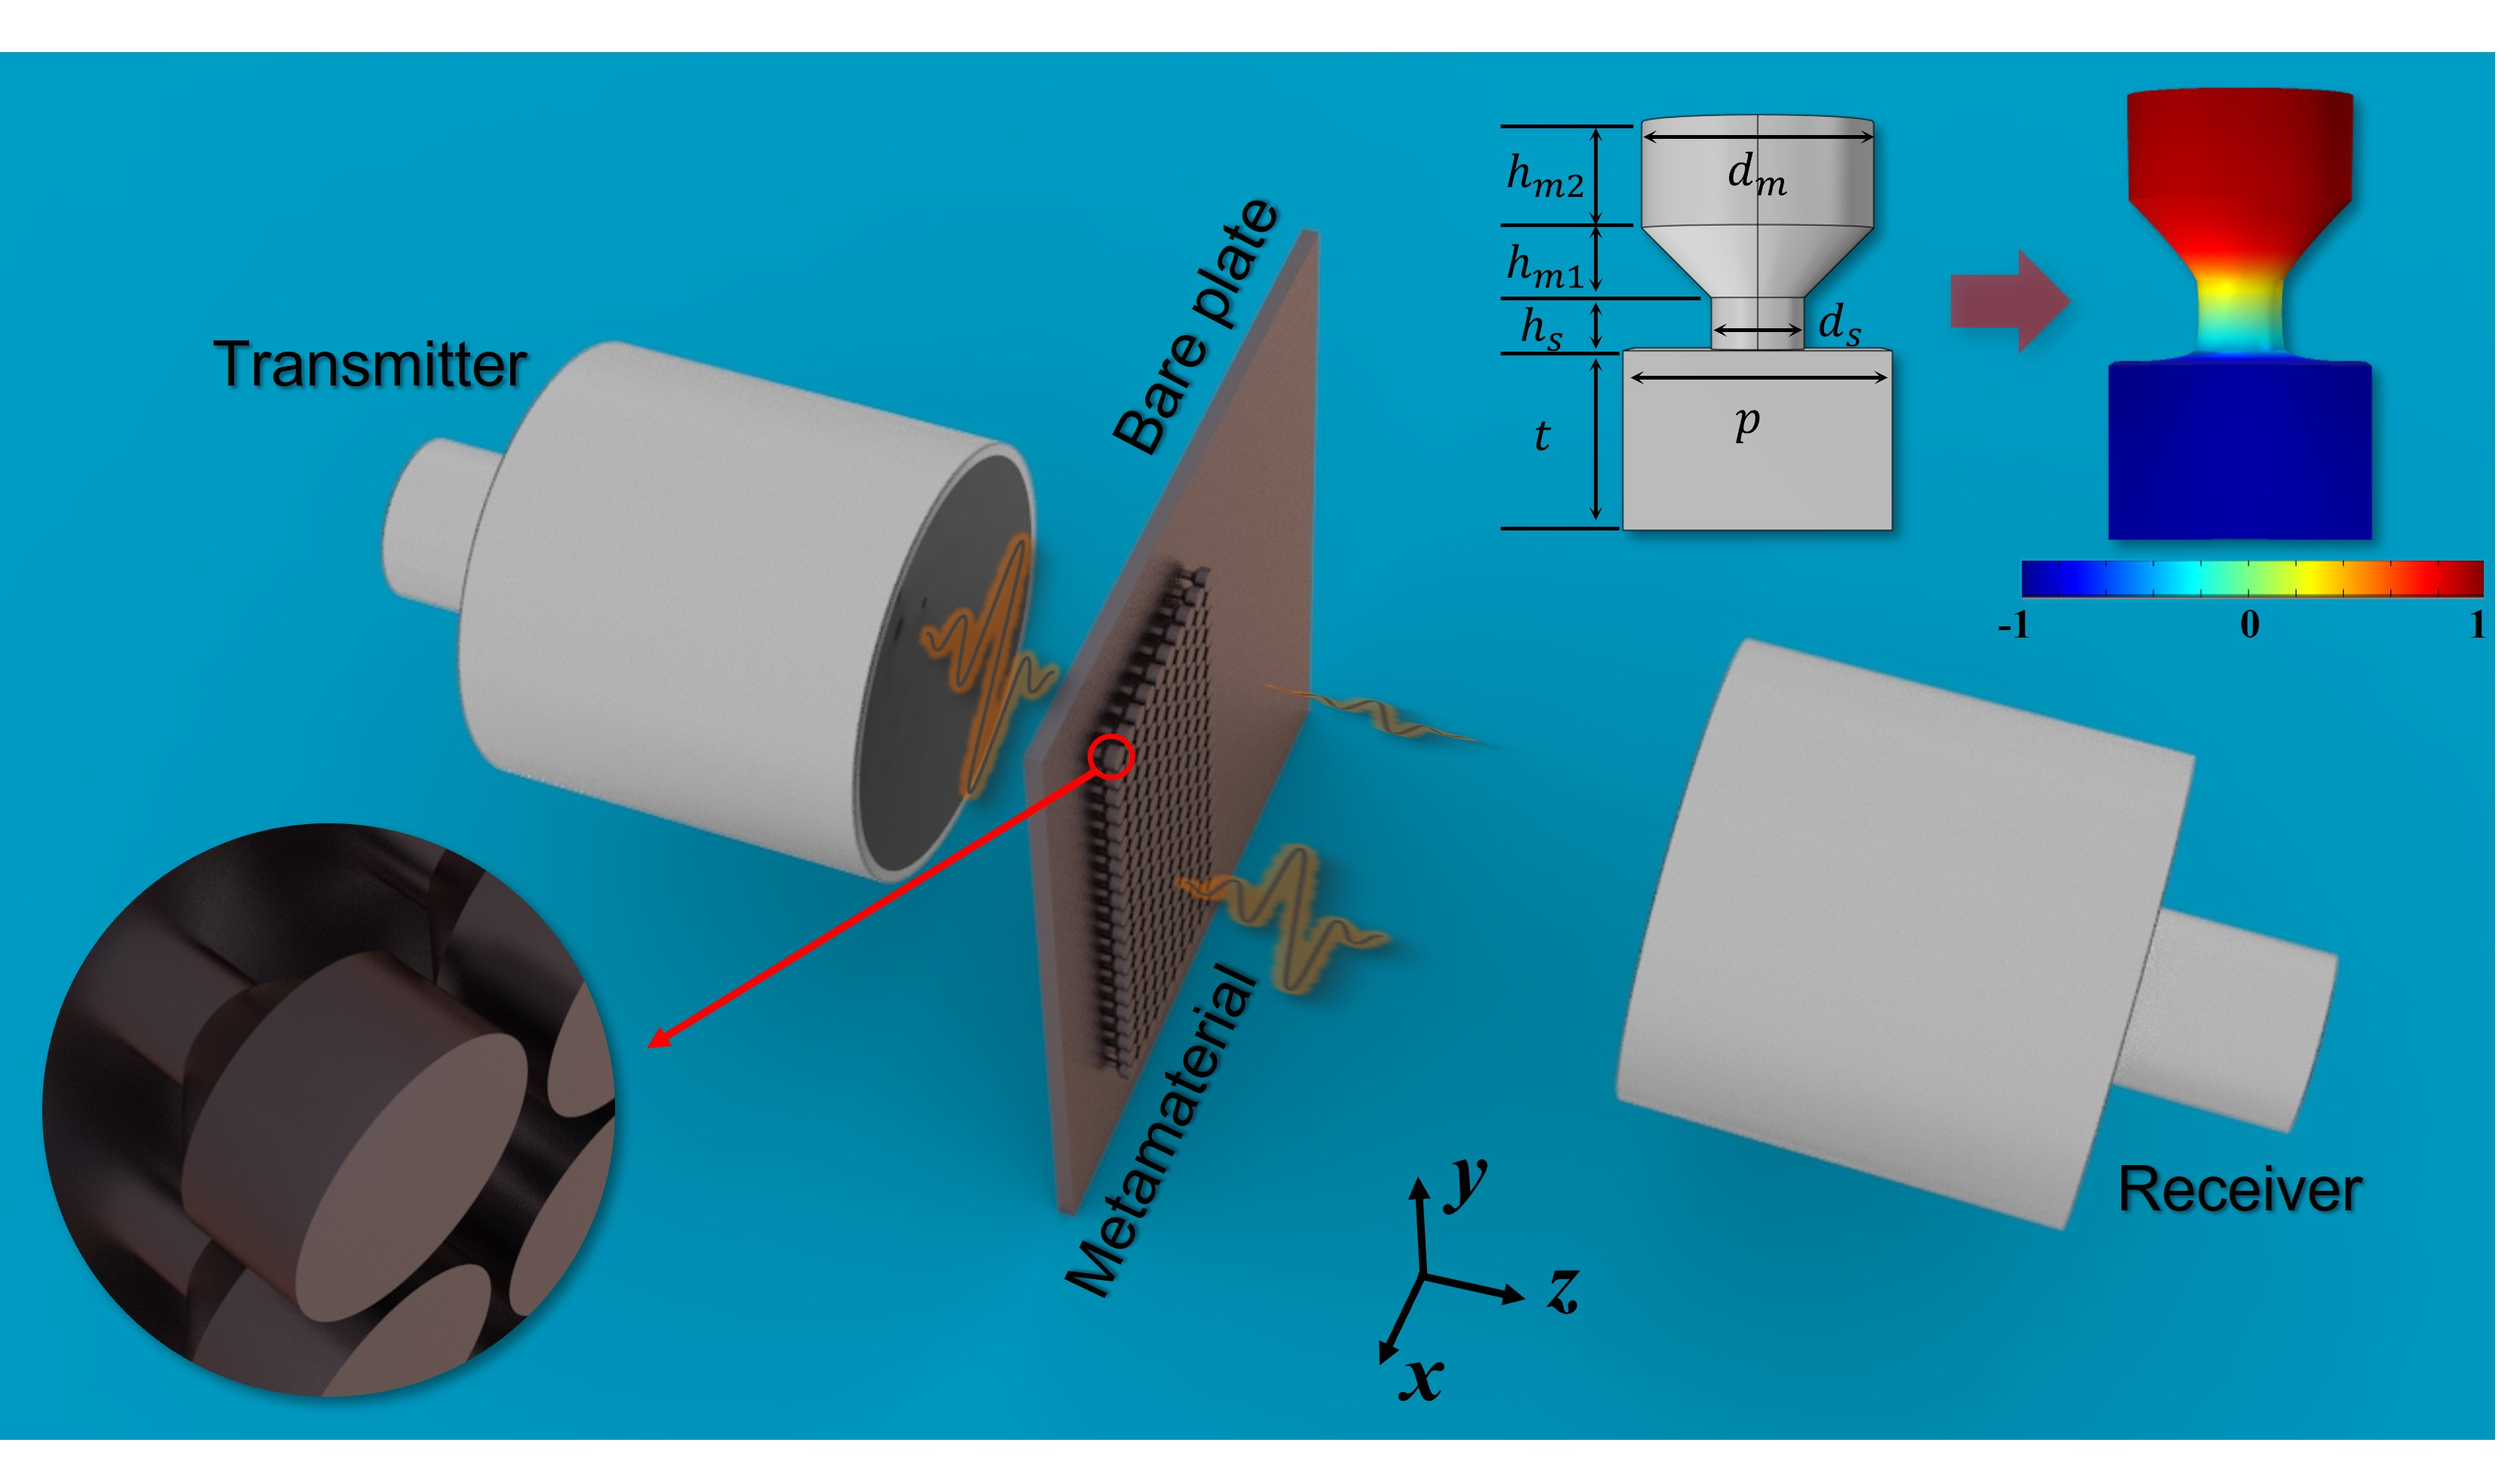
\includegraphics[width=\linewidth]{Figure1.jpg}
  \caption{Figure 1 caption goes here. Reproduced with permission.\textsuperscript{[Ref.]} Copyright Year, Publisher. }
  \label{fig:boat1}
\end{figure}

\begin{figure}
  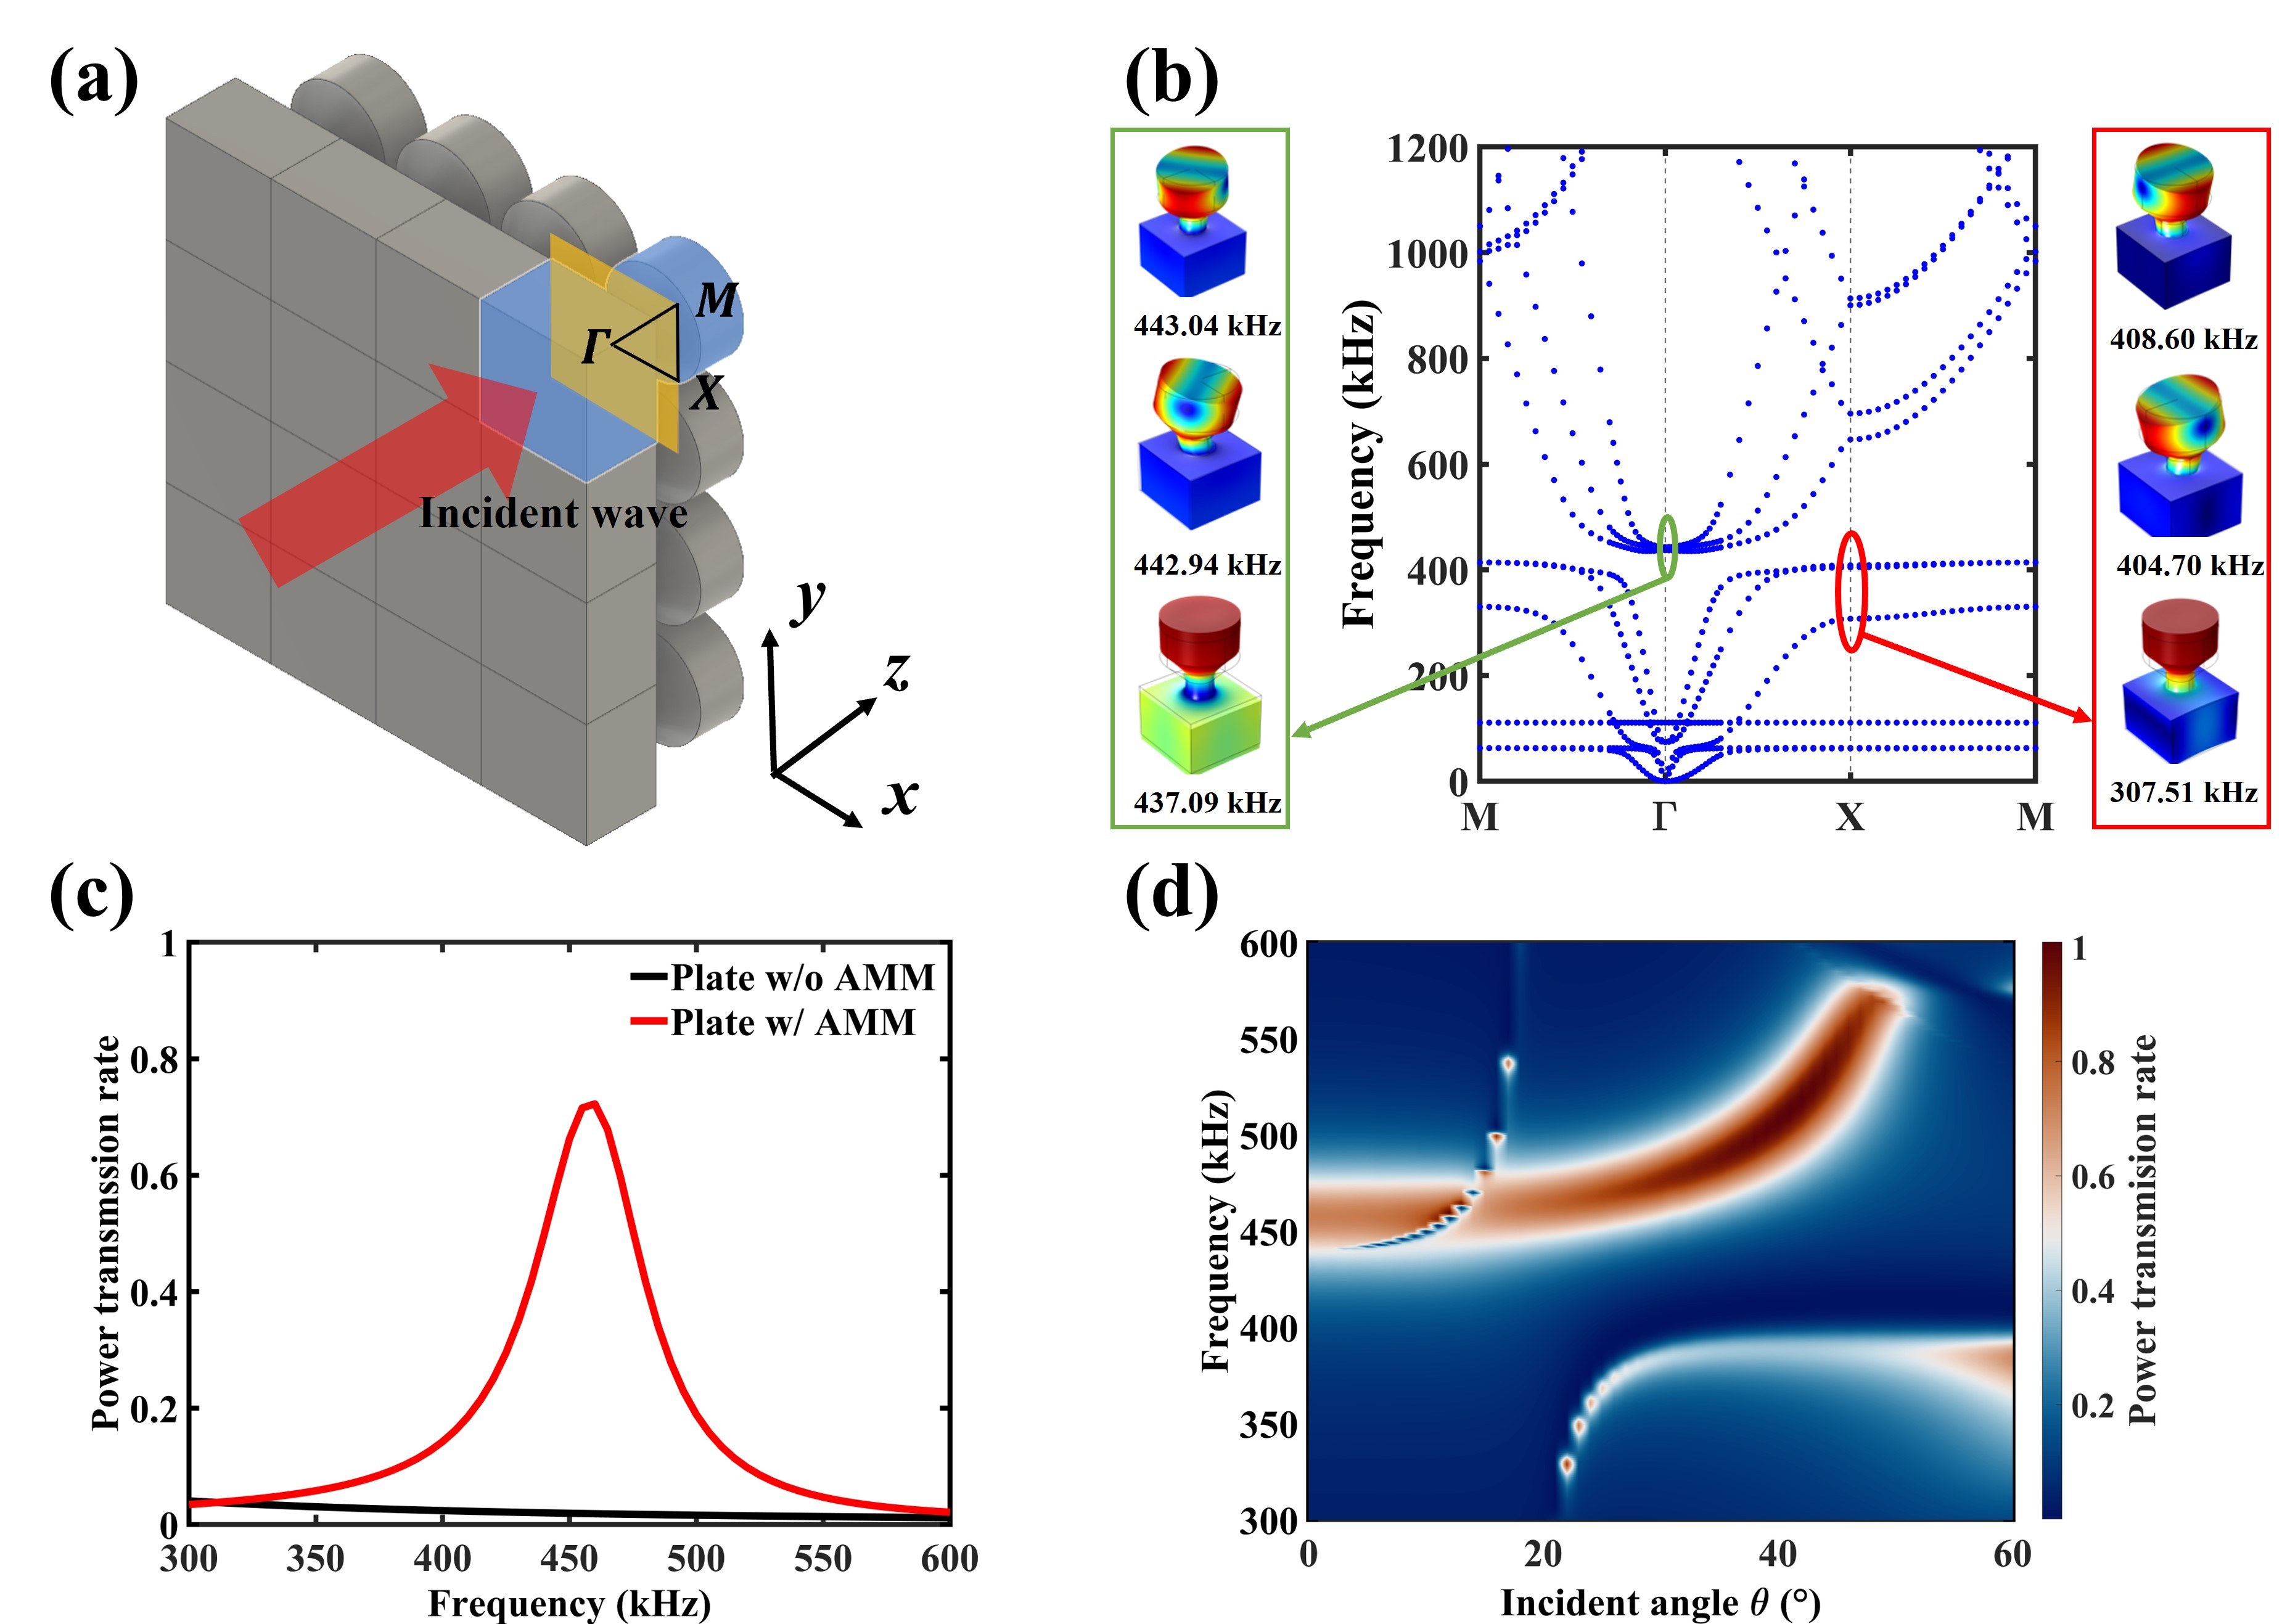
\includegraphics[width=\linewidth]{Figure2.jpg}
  \caption{Figure 2 caption goes here. Reproduced with permission.\textsuperscript{[Ref.]} Copyright Year, Publisher.}
  \label{fig:boat1}
\end{figure}

\begin{figure}
  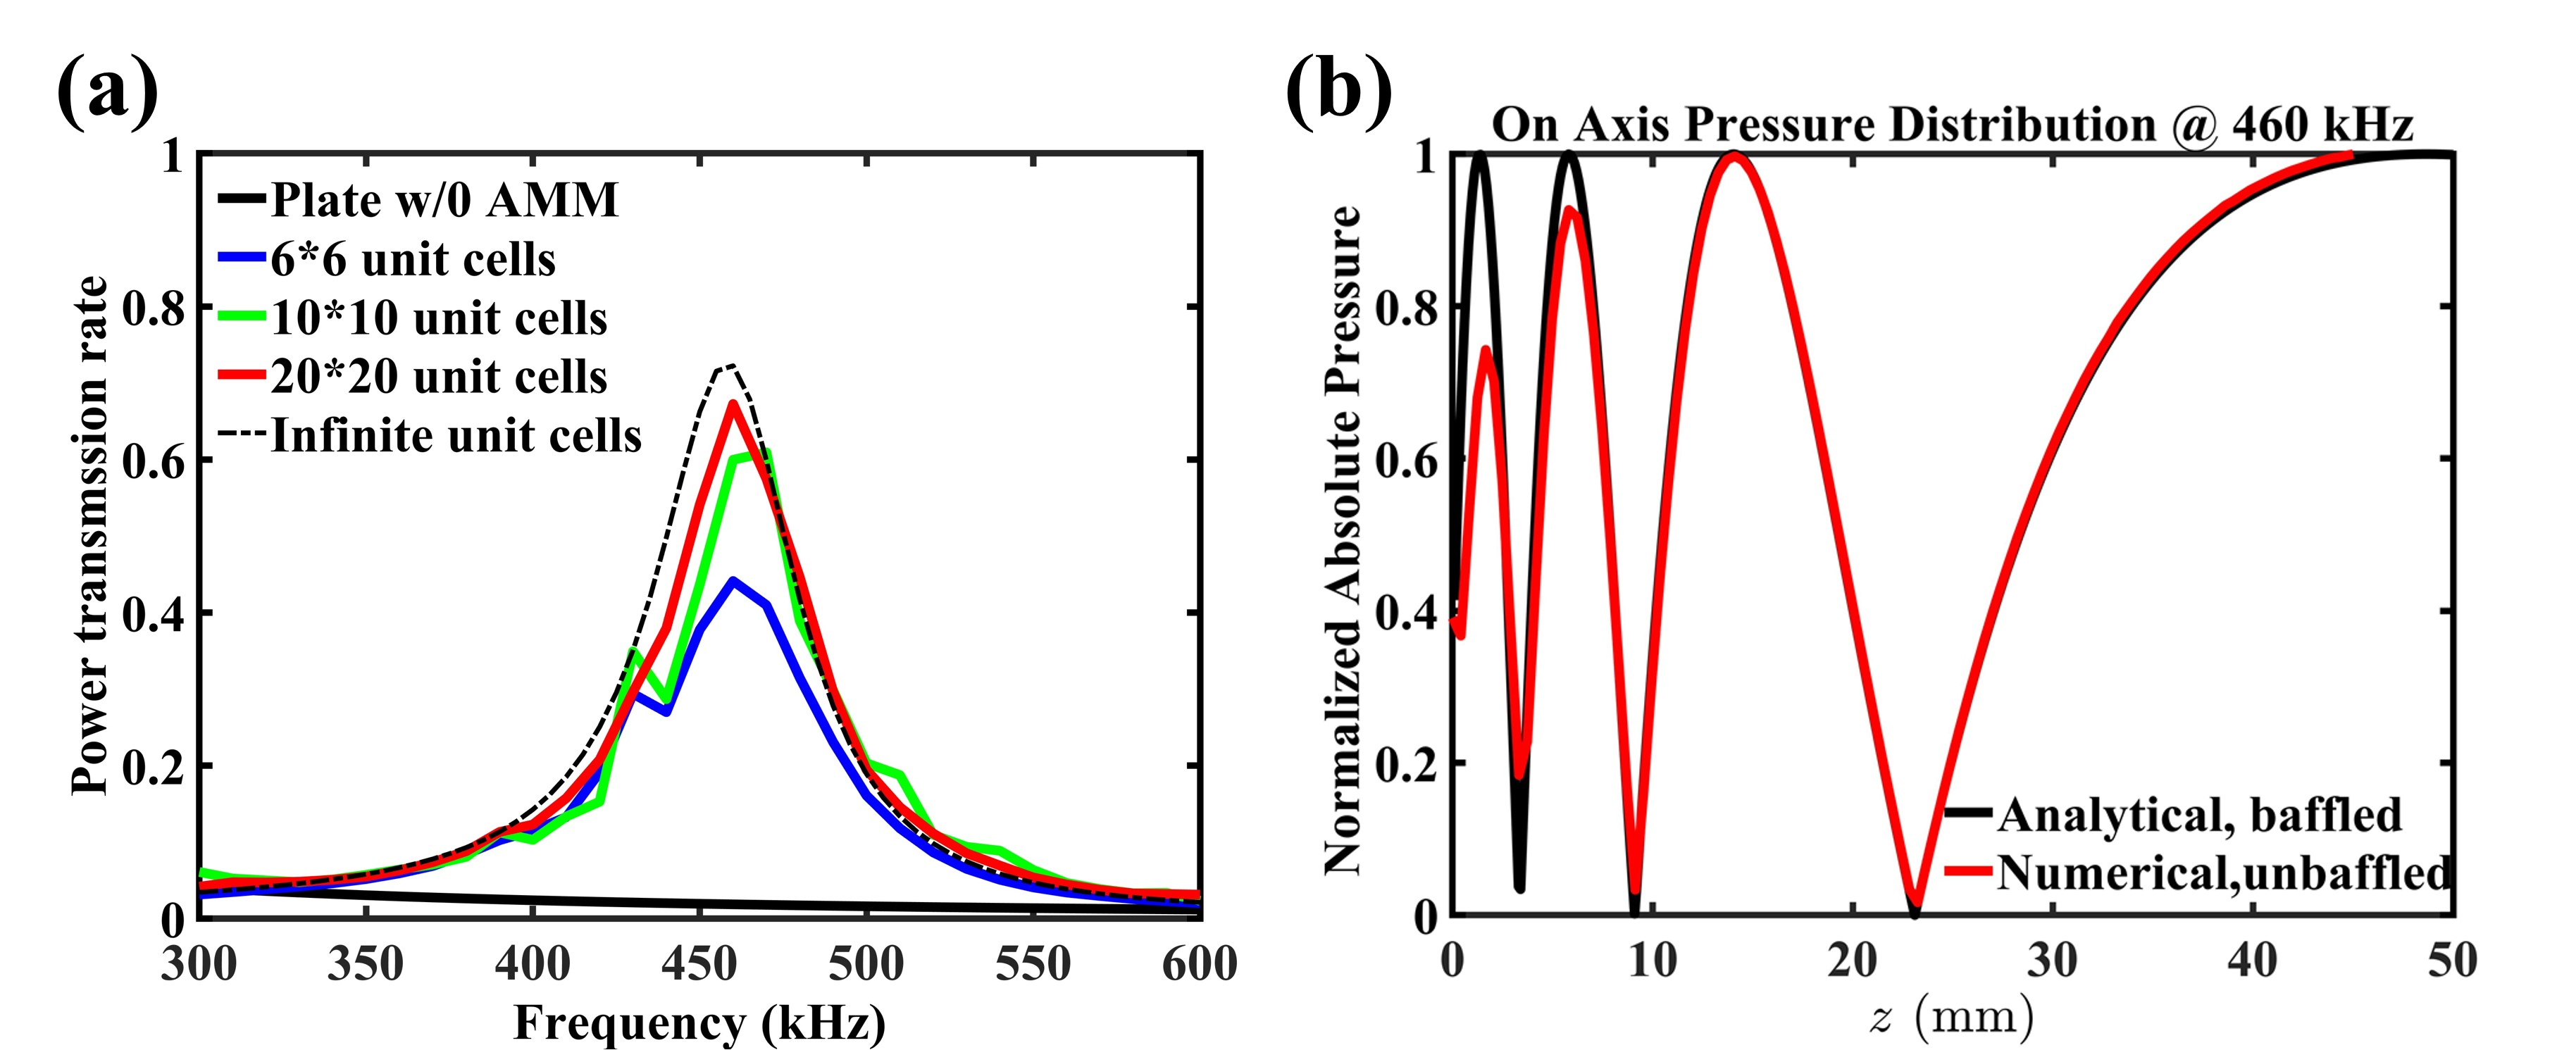
\includegraphics[width=\linewidth]{Figure3.jpg}
  \caption{Figure 3 caption goes here. Reproduced with permission.\textsuperscript{[Ref.]} Copyright Year, Publisher.}
  \label{fig:boat1}
\end{figure}

\begin{figure}
  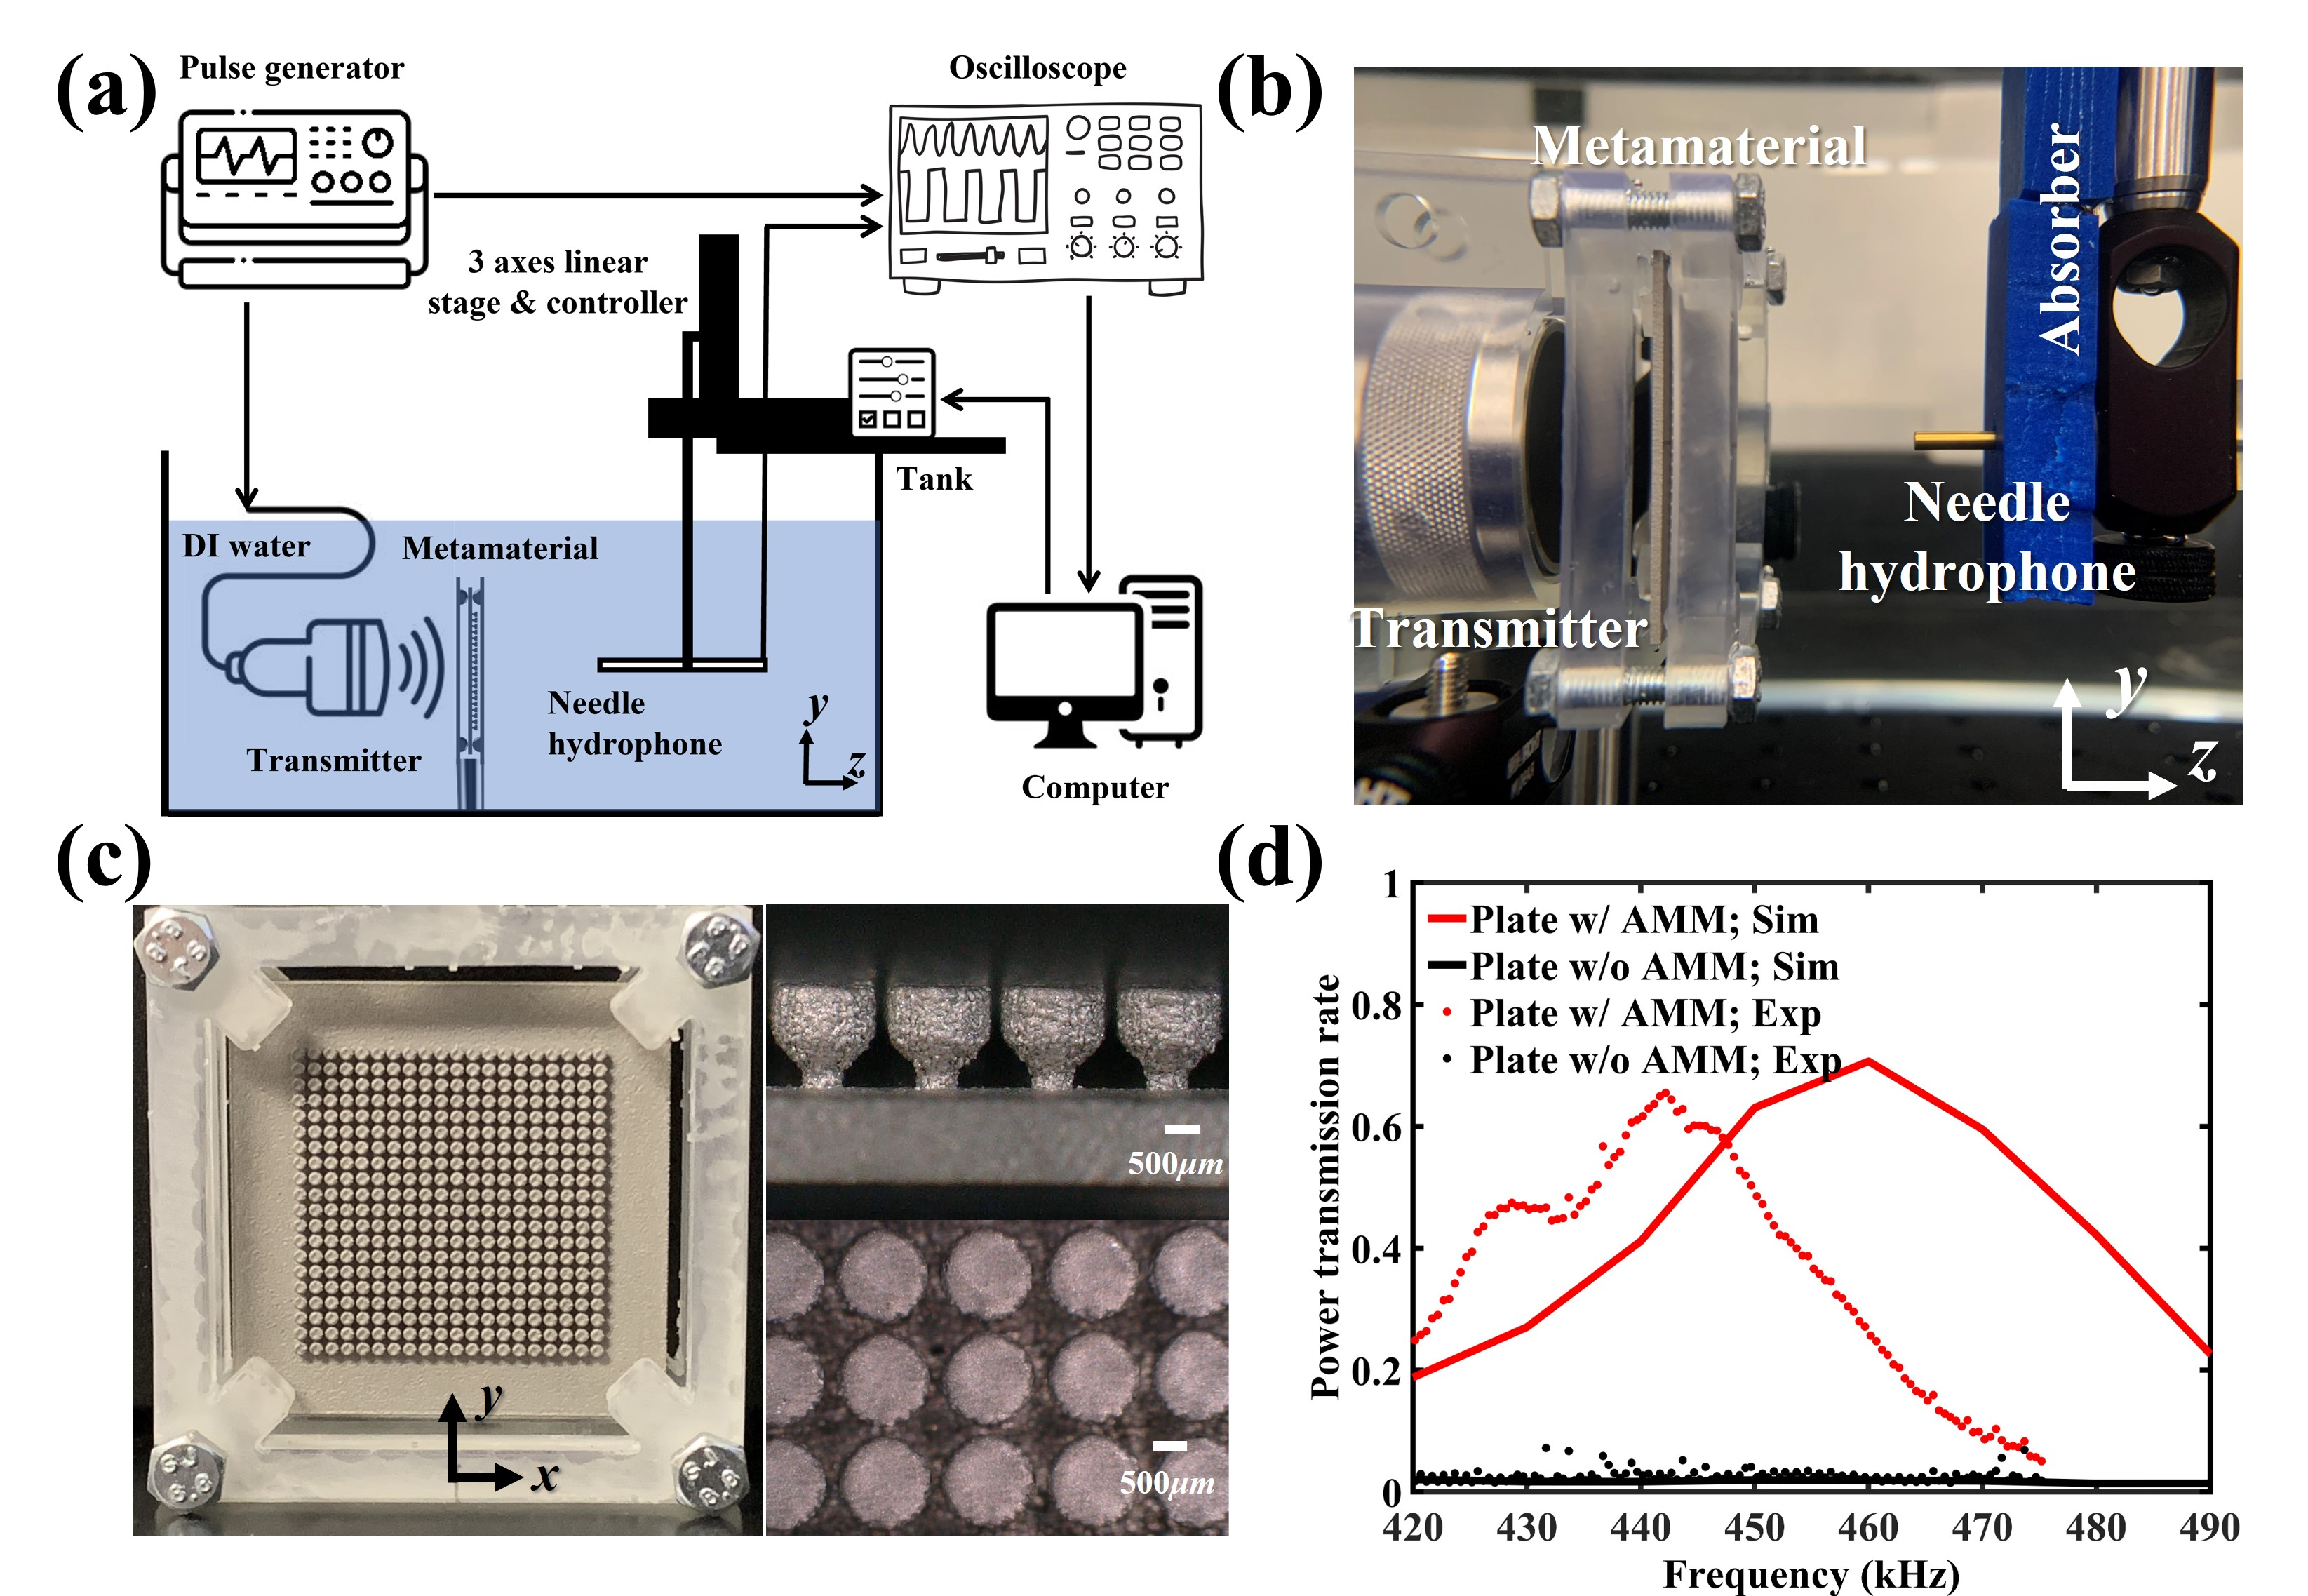
\includegraphics[width=\linewidth]{Figure4.jpg}
  \caption{Figure 4 caption goes here. Reproduced with permission.\textsuperscript{[Ref.]} Copyright Year, Publisher.}
  \label{fig:boat1}
\end{figure}

\begin{figure}
  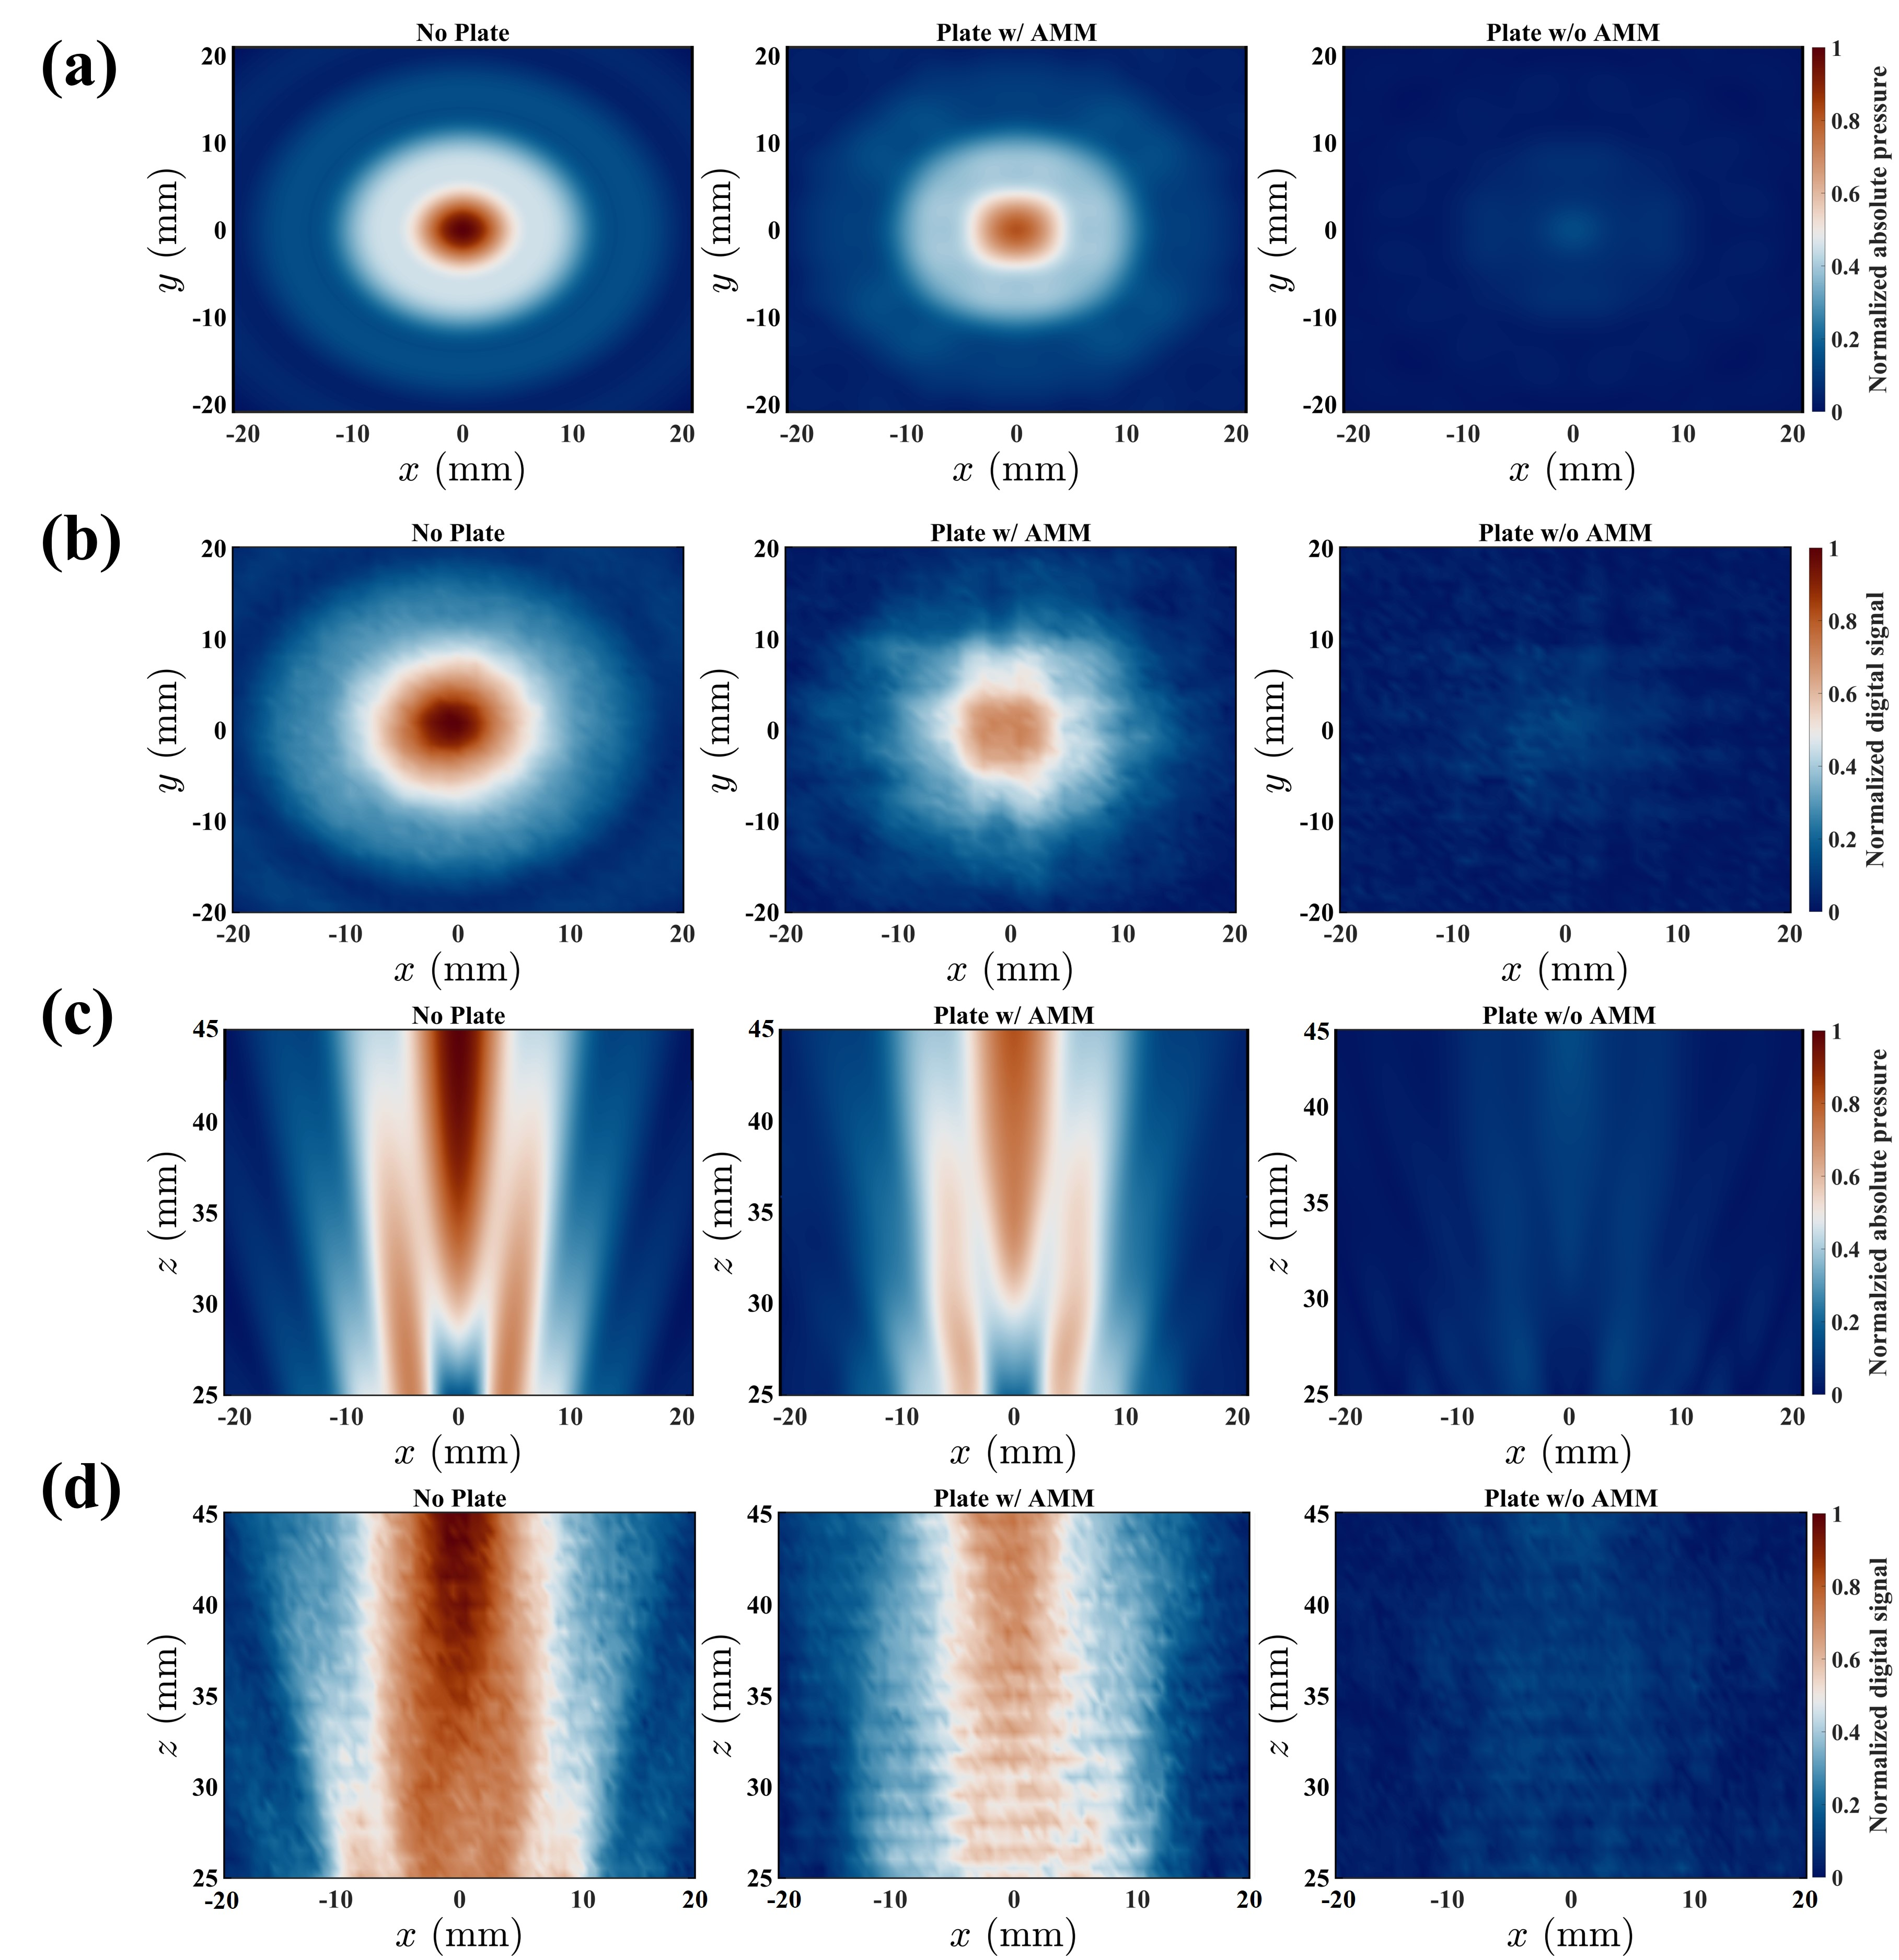
\includegraphics[width=\linewidth]{Figure5V2.jpg}
  \caption{Figure 5 caption goes here. Reproduced with permission.\textsuperscript{[Ref.]} Copyright Year, Publisher.}
  \label{fig:boat1}
\end{figure}




\subsection{Wireless power charging}

\begin{figure}
  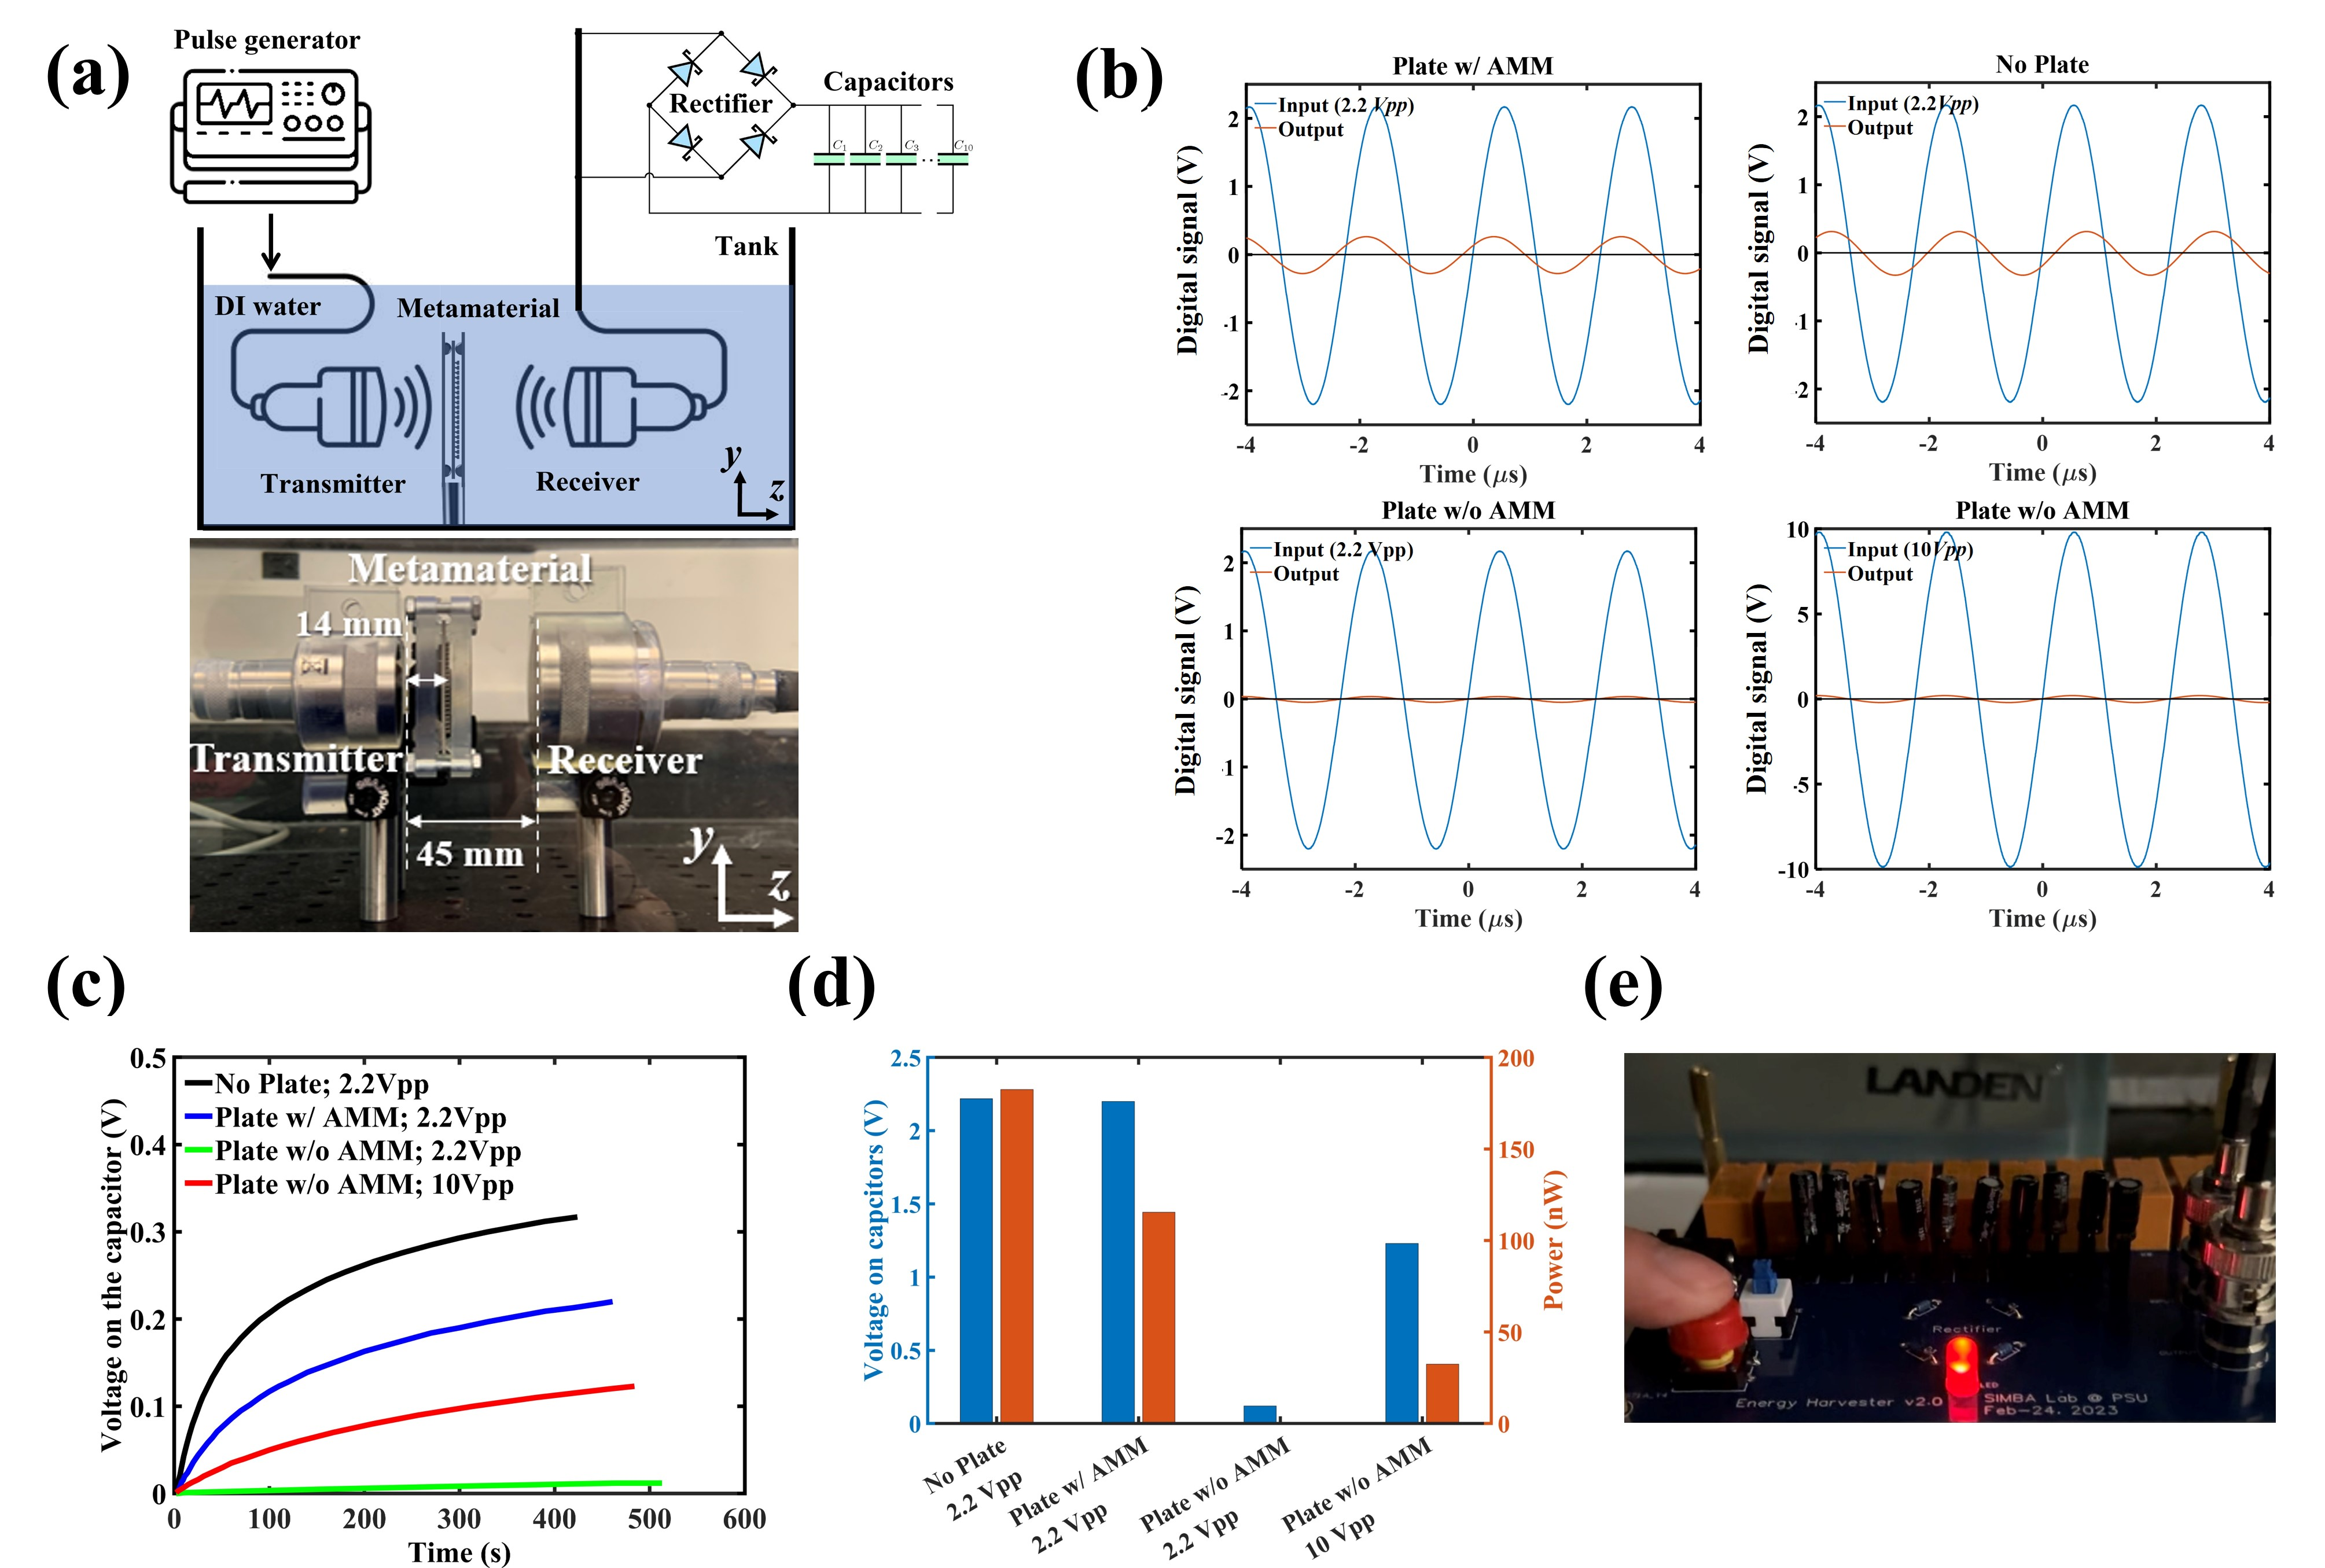
\includegraphics[width=\linewidth]{Figure6.jpg}
  \caption{Figure 6 caption goes here. Reproduced with permission.\textsuperscript{[Ref.]} Copyright Year, Publisher.}
  \label{fig:boat1}
\end{figure}



\section{Conclusion}

% Experimental section

\section{Experimental Section}
\threesubsection{Numerical Simulations}\\
\threesubsection{Fabrication}\\
\threesubsection{Energy Harvesting Circuit}\\
(See Note S3 in the Supporting Information)\\
\threesubsection{Experimental Measurements}\\


\medskip
\textbf{Supporting Information} \par %Please delete the Suppporting Information statement if it is not applicable. Please supply Supporting Information in another file. Supporting information should not be provided in .tex format
Supporting Information is available from the Wiley Online Library or from the author.



% Acknowledgements
\medskip
\textbf{Acknowledgements} \par %delete if not applicable))
J.J., H.H., and J.Z equally contributed to this work. Y.J. thanks the NSF for supports through CMMI 2119545, 1951221, and 2039463.

% References
\medskip

% Use the following code if you wish to generate your bibliography with BibTeX;
% replace the string "MSP-template" below with the name(s) of
% the BibTeX data base(s) you want to use.
% The resulting bibliography-output (the content of the .bbl file)
% must be pasted back into this file before submission.
% Please also include your BibTeX data base file(s) in your submission
% so that we can re-run BibTeX if necessary.
%
\bibliographystyle{MSP}
\bibliography{ref}






% Figures/tables and captions
% Permission statements are required for all figures reproduced or adapted from previously published articles/sources. Please also ensure that all necessary permissions to reproduce images have been received
% Please remove these statements for original figures


\begin{table}
 \caption{Table 1 caption}
  \begin{tabular}[htbp]{@{}lll@{}}
    \hline
    Description 1 & Description 2 & Description 3 \\
    \hline
    Row 1, Col 1  & Row 1, Col 2  & Row 1, Col 3  \\
    Row 2, Col 1  & Row 2, Col 2  & Row 2, Col 3  \\
    \hline
  \end{tabular}
\end{table}


% Table of contents entry should be 50 - 60 words long
% Image should be 55 mm broad and 50 mm high or 110 mm broad and 20 mm high

\begin{figure}
\textbf{Table of Contents}\\
\medskip
  
\includegraphics{toc-image.png}
  \medskip
  \caption*{ToC Entry}
\end{figure}

\end{document}
